\section{Experimentation\label{se:imp}}
We have implemented the MOHA in C++. %, and  compiled by gcc 4.8.1. 
The efficiency of the algorithm over the constraint model has been evaluated with realistic benchmarks, including an H264 decoder~\cite{IEICE14}, a TMNR~\cite{cotton2011multi}, a Multi-Window Display (MWD) application~\cite{atienza2008},  a Livermore Loop and a Bufferfly ~\cite{kessler2009optimized}, and an MP3 decoder. %Ultrasound~\cite{wang2014case}. 

\begin{table}[htp]\centering
\caption{Experimental parameters \label{tab:setting}}
\begin{lrbox}{\tablebox}
\begin{tabular}{l l }
\hline
	Items & Value \\
\hline
the number of iterations for stopping criterion & 500  \\
the size of population  &100 \\
the size of elitist population & 100 \\
non-updated times & $number\_of\_tasks/3 $\\
execution possibility of mutation operator & 0.1 \\
the ratio of the probability of two perturbations	& 1:1 \\
\hline
\end{tabular}	
\end{lrbox}
\scalebox{0.8}{\usebox{\tablebox}}
\end{table}

All the experiments are performed on a PC with intel 2.2 GHz processor and 8.0 GB memory. The detailed parameters in MOHA are listed in Table \ref{tab:setting}. 

%The stopping criterion is that the number of iterations reaches 500 times, and the size of population is 100 for a wider exploration. Meanwhile, the elitist population is set as 100. Another important parameter is the number of non-updated times in local search phase, which is dynamically set as $ \frac{number\_of\_tasks}{3} $. The mutation operator is executed with a possibility of 0.1 and the two perturbations proceed with an equal probability. 

\subsection{Efficiency comparison with classical methods}

\begin{figure}[htp]
\centering

\subfigure[H264 with 2 processors\label{fig:h264:2}]{
 \begin{minipage}[b]{0.25\textwidth}
  \scalebox{0.045}{\rotatebox{0}{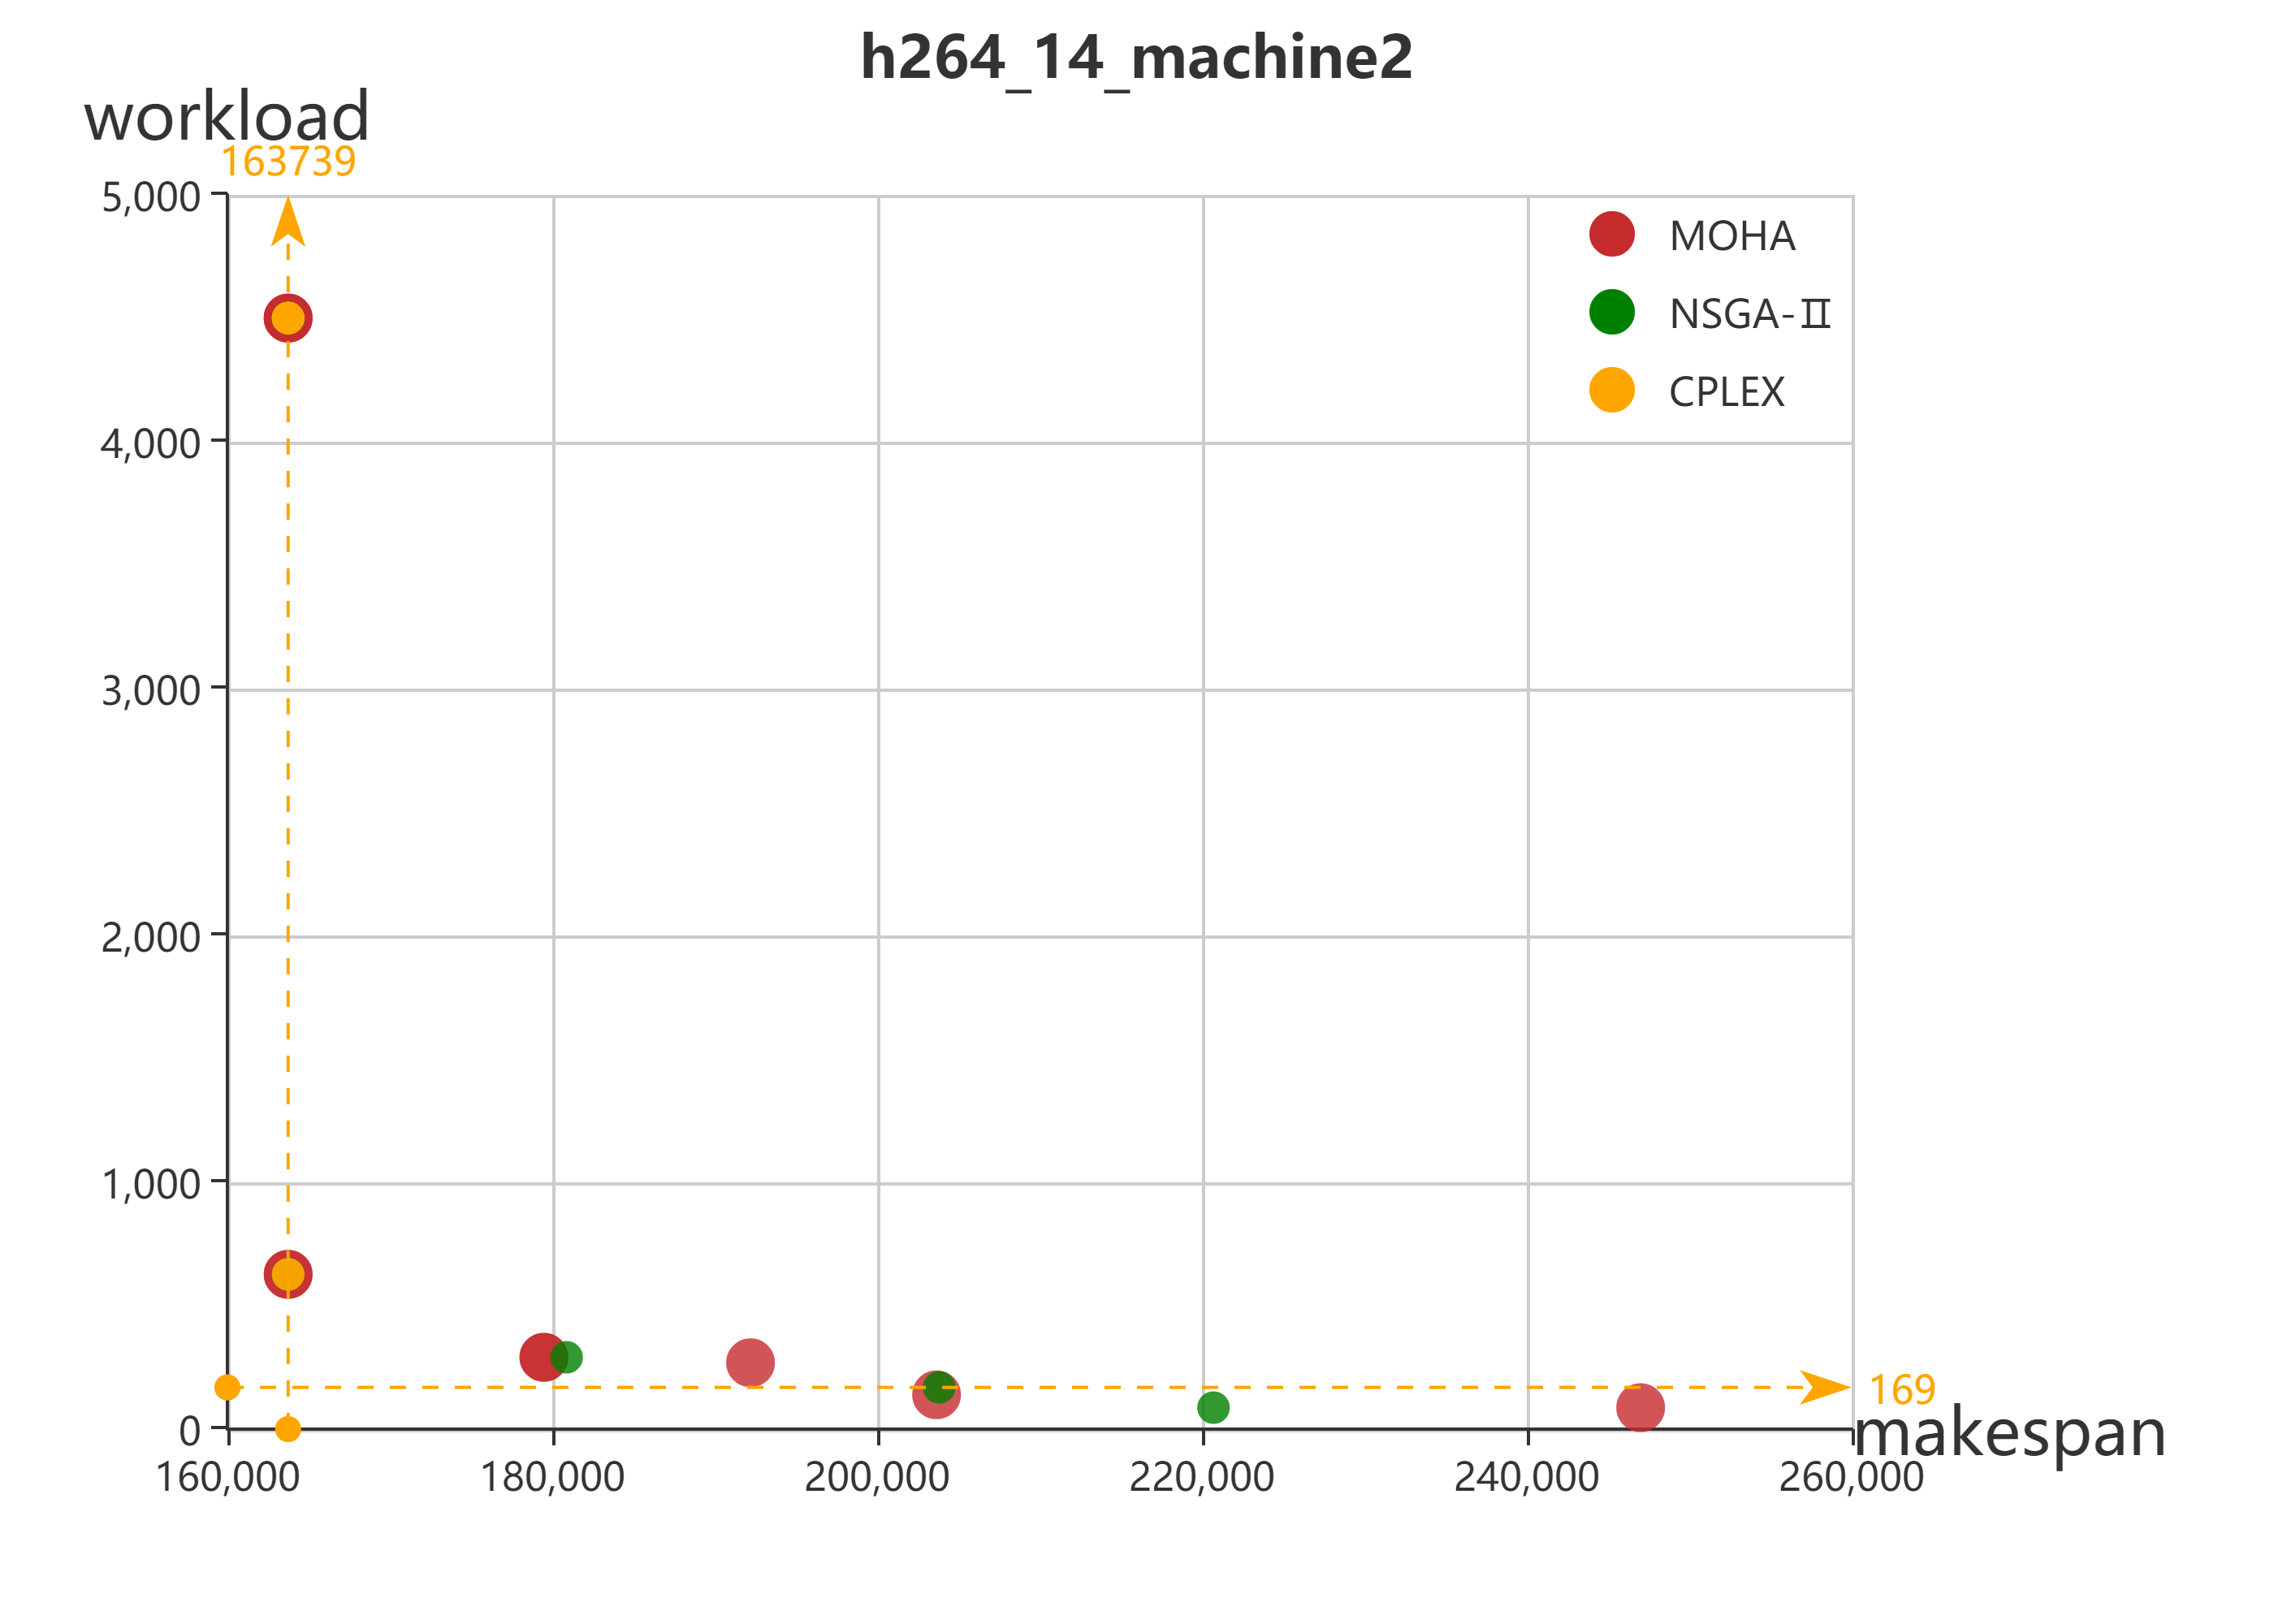
\includegraphics{./figures/h264_14_machine2}}}
\end{minipage}}%
\subfigure[H264 with 4 processors\label{fig:h264:2}]{
\begin{minipage}[b]{0.25\textwidth}
  \scalebox{0.045}{\rotatebox{0}{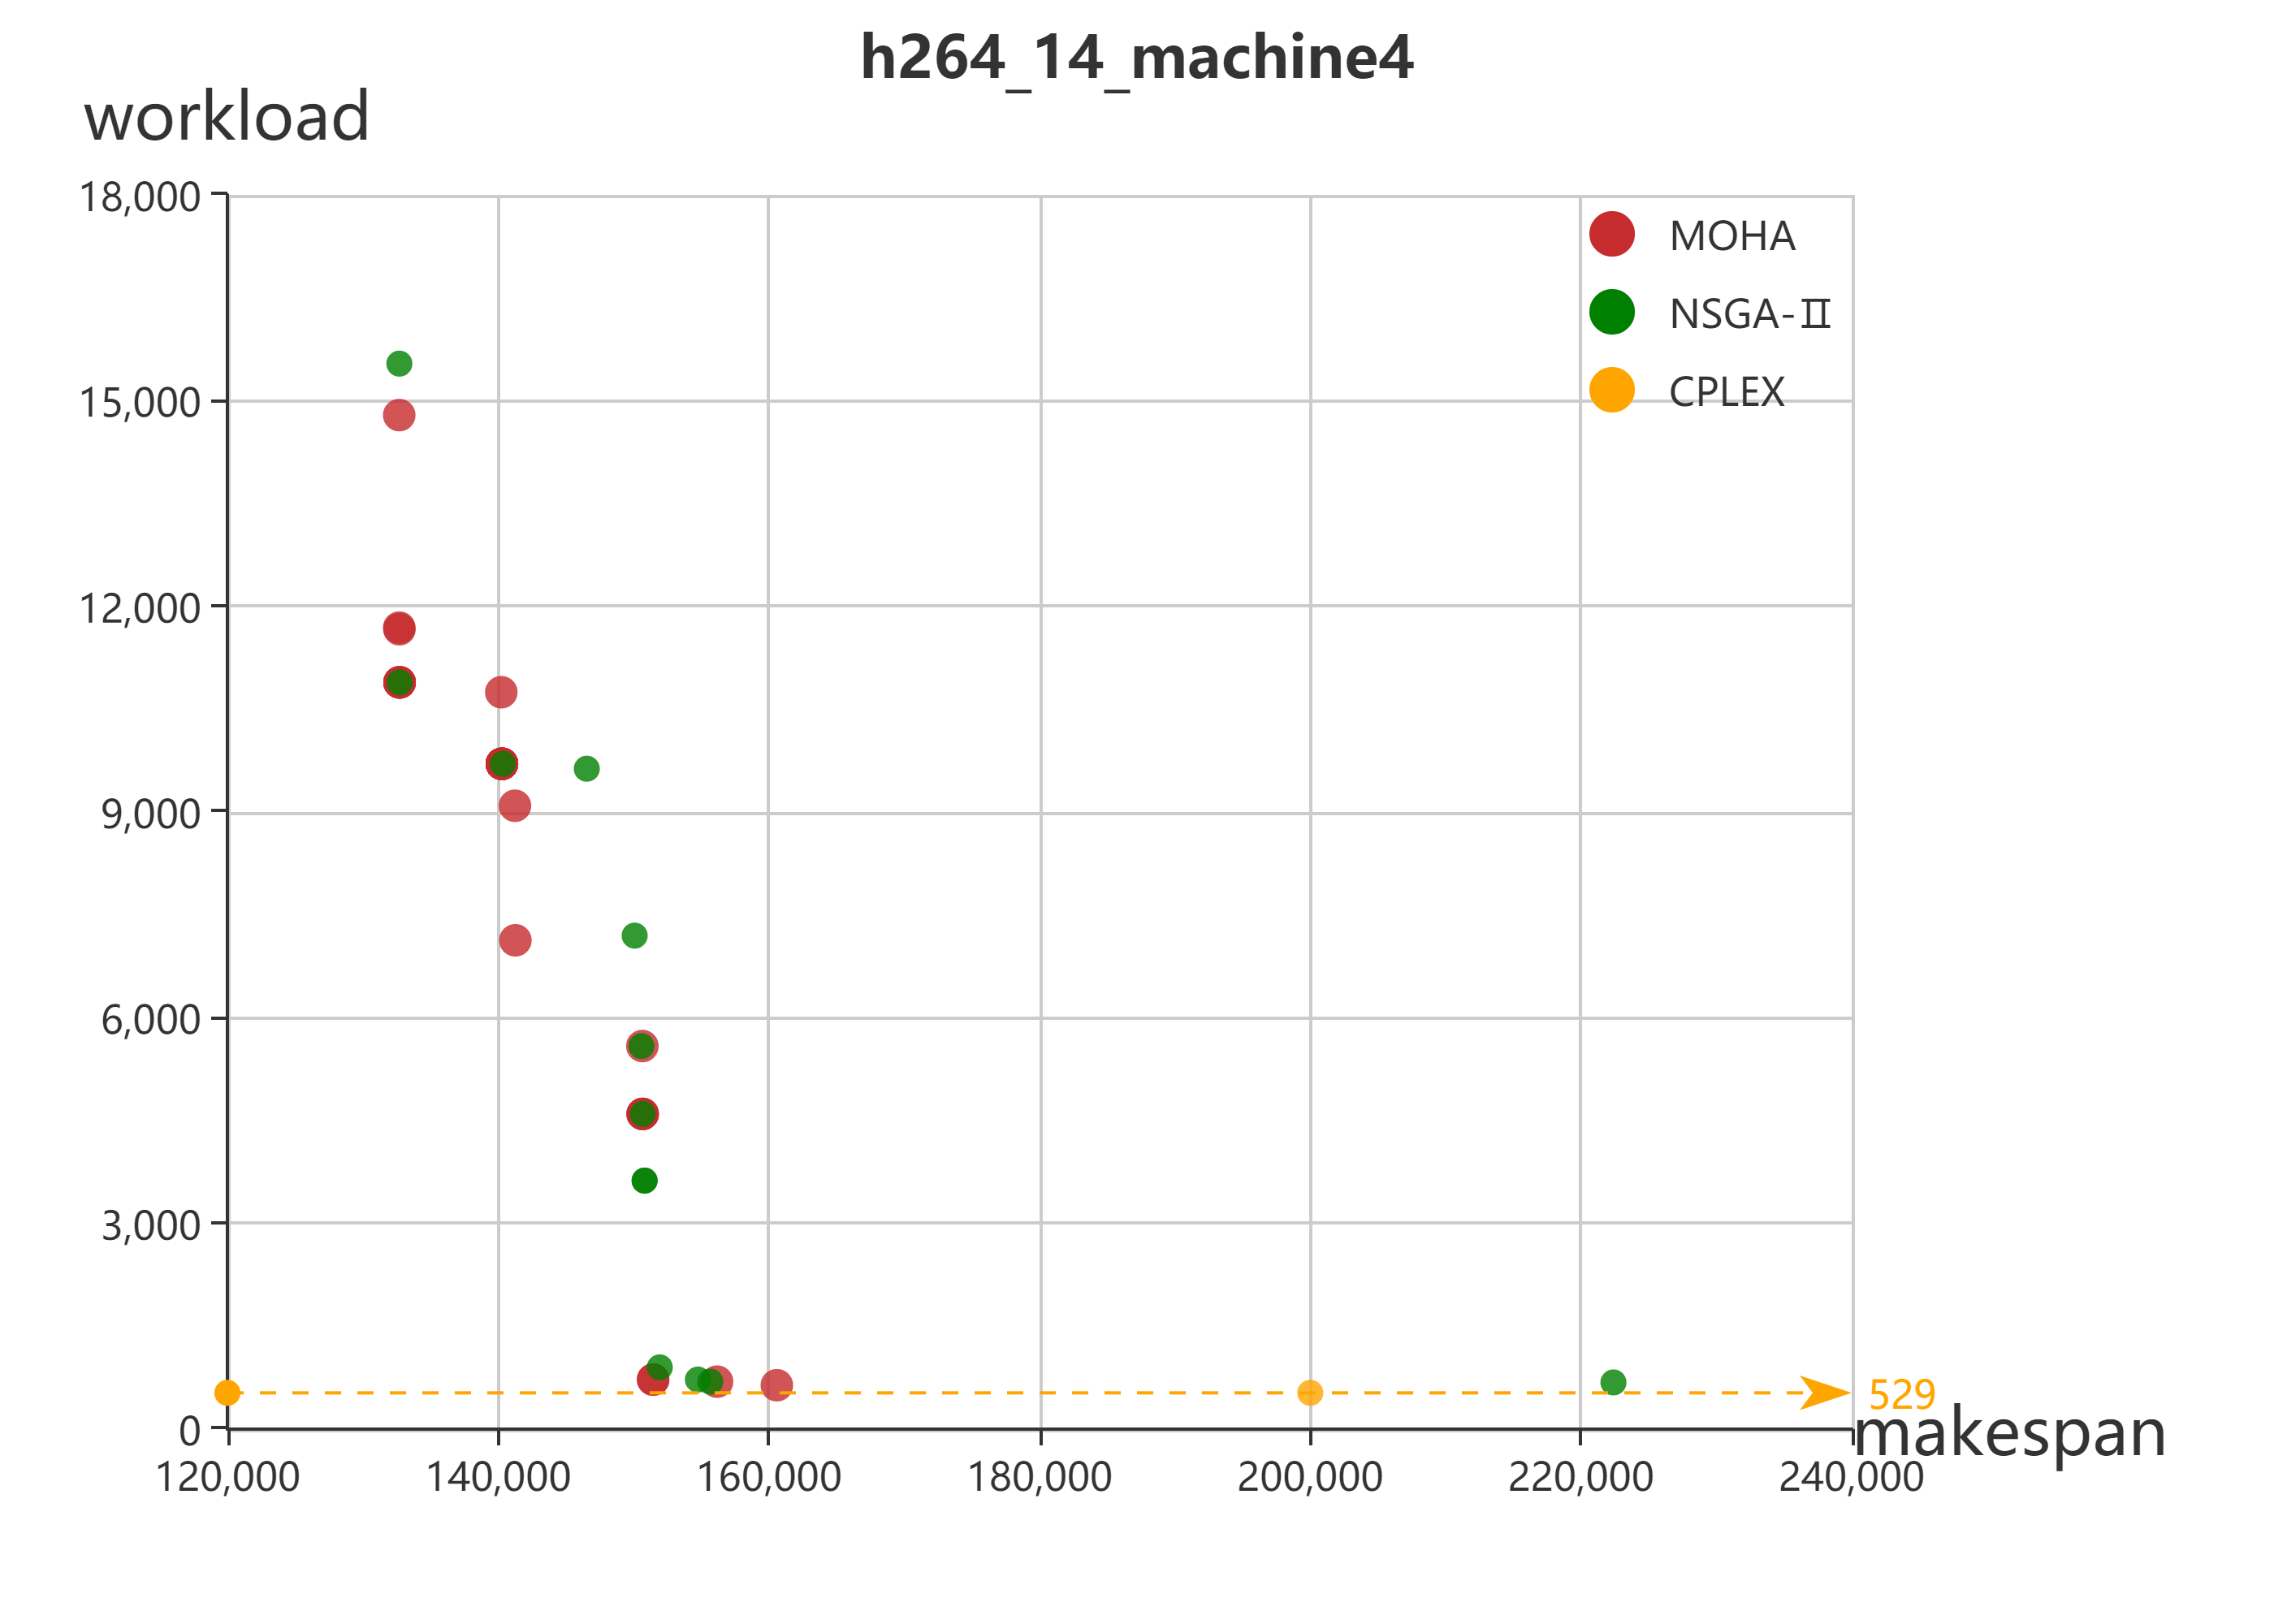
\includegraphics{./figures/h264_14_machine4}}}
\end{minipage}}
\caption{\label{fig:distribution} Distribution of final sets obtained by MOHA and NSGAII}
 \end{figure} 

%\begin{figure}[htp]
%\centering
%
%\subfigure[H264 with 2 processors\label{fig:h264}]{
% %\begin{minipage}[b]{0.25\textwidth}
%  \scalebox{0.065}{\rotatebox{0}{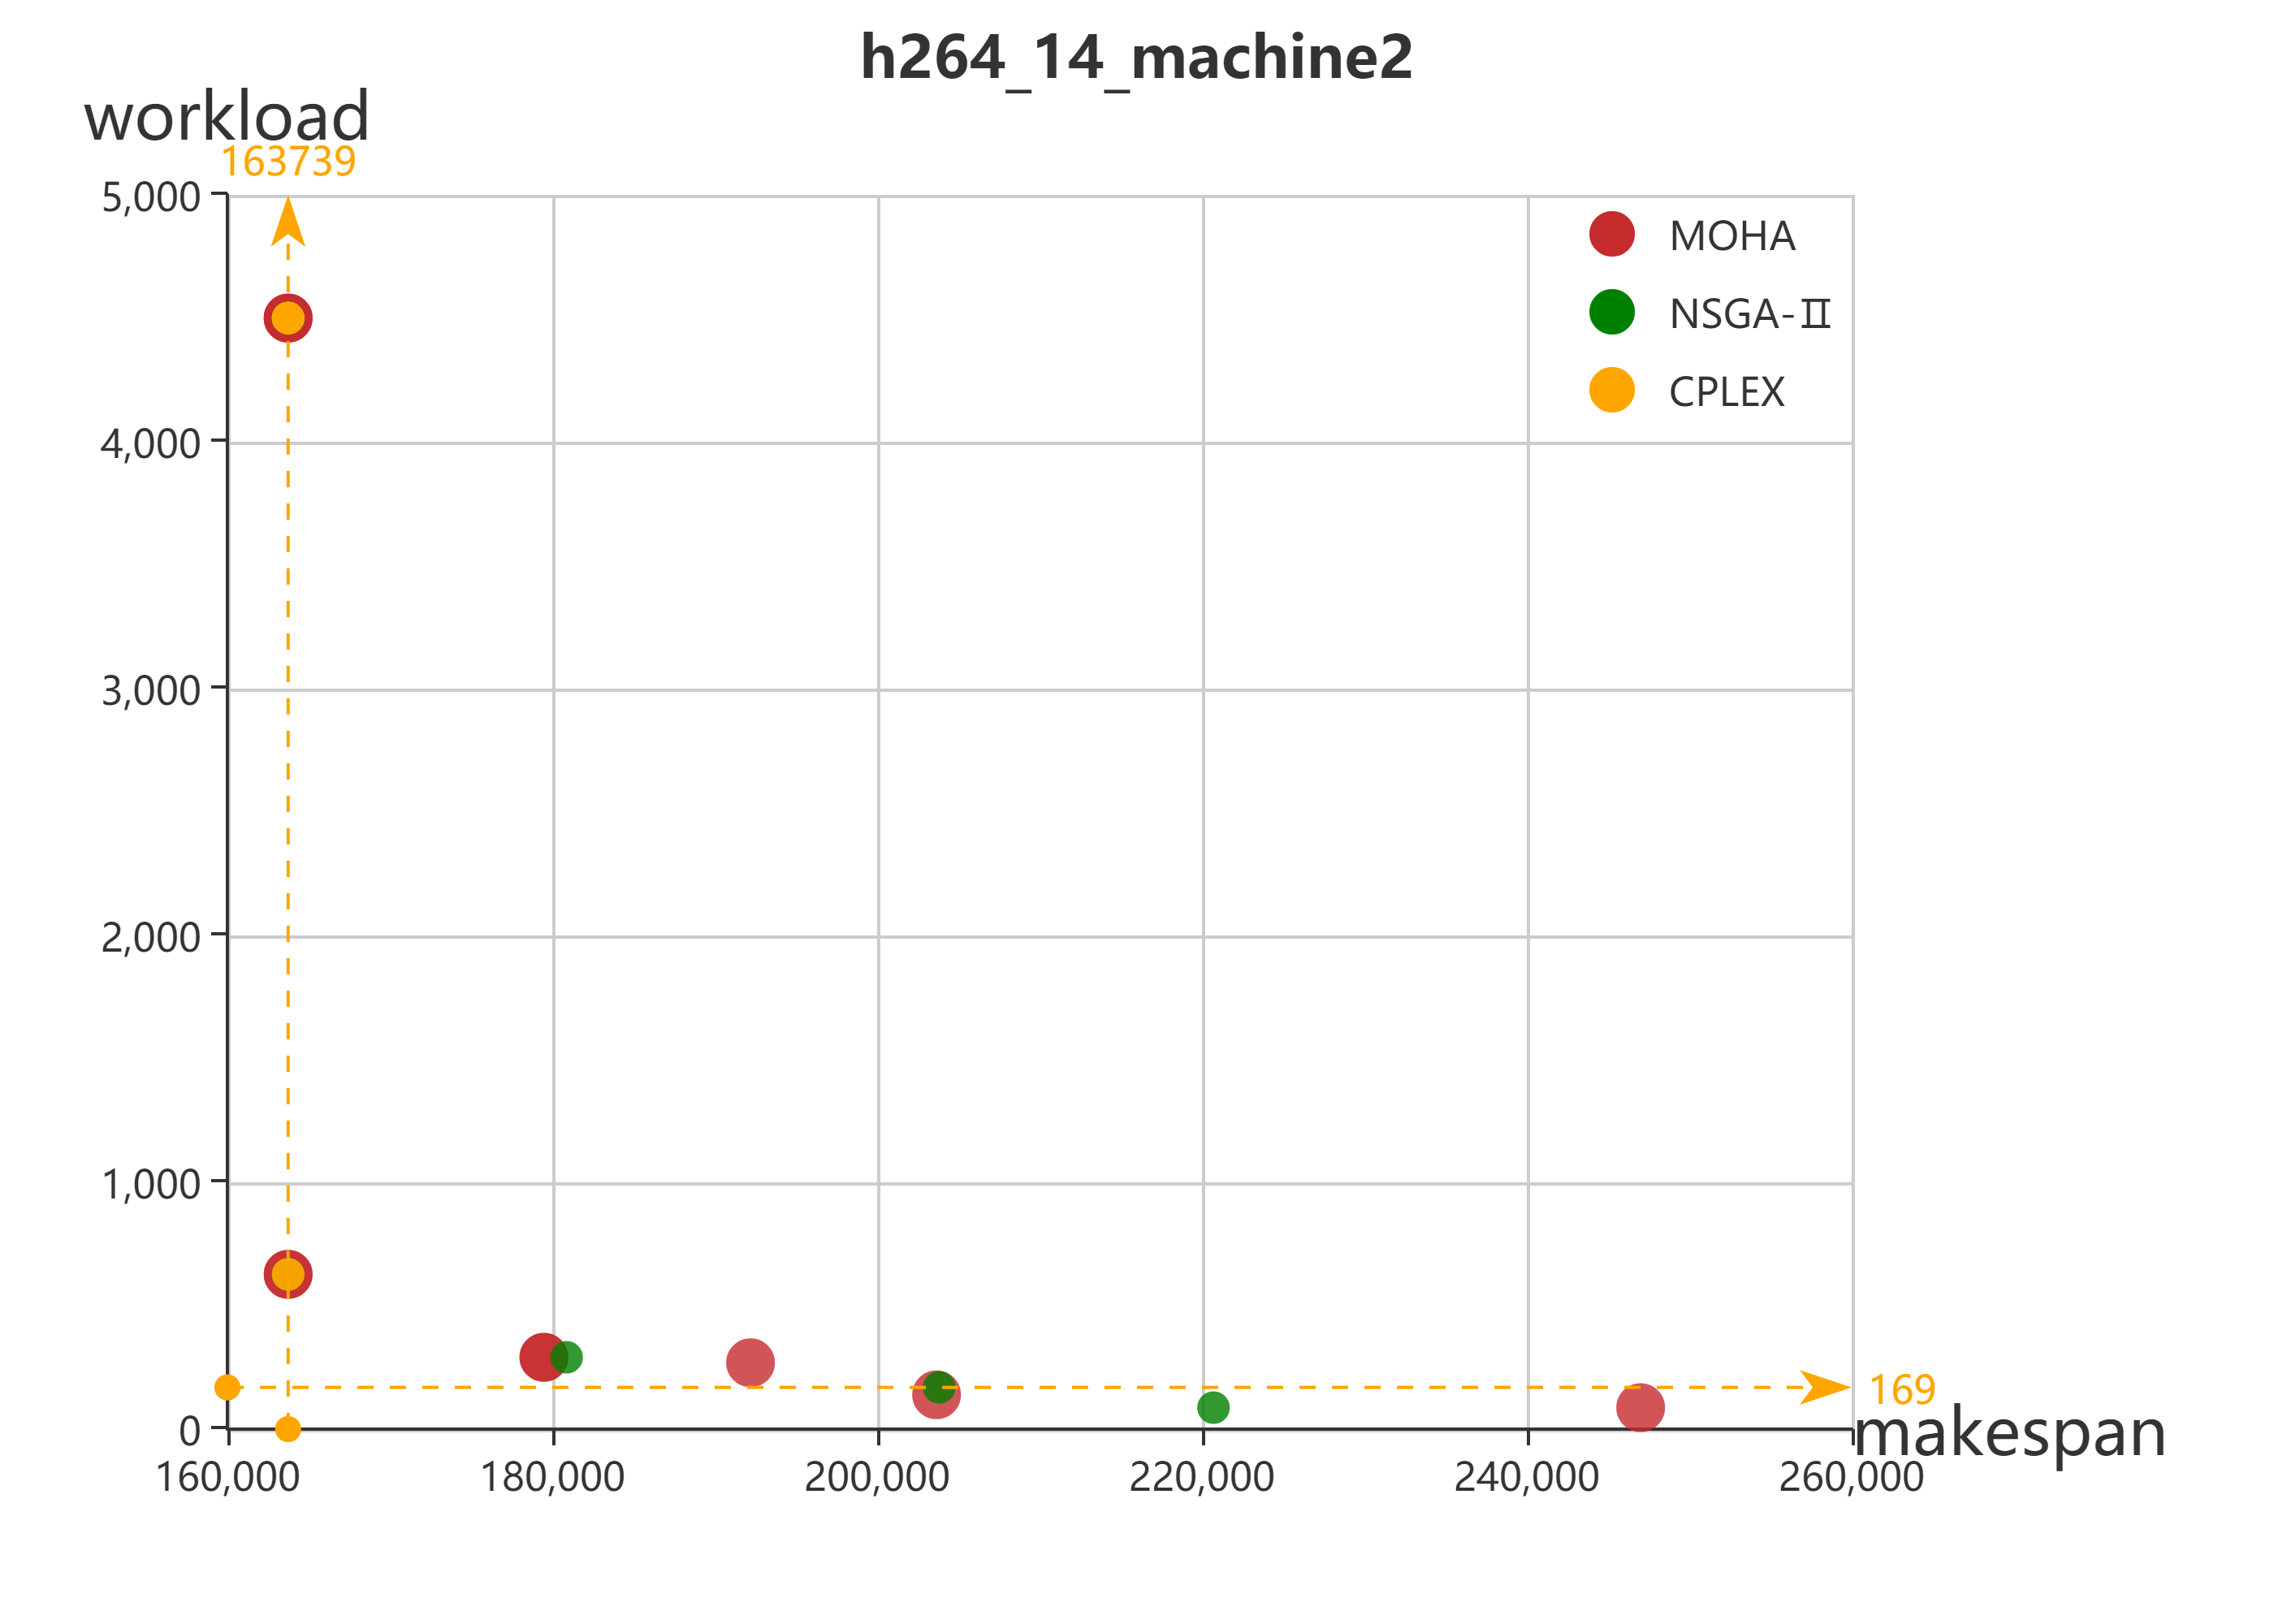
\includegraphics{./figures/h264_14_machine2}}}
%  }
%%\end{minipage}\
%\subfigure[H264 with 4 processors]{
%%\begin{minipage}[b]{0.25\textwidth}
%  \scalebox{0.065}{\rotatebox{0}{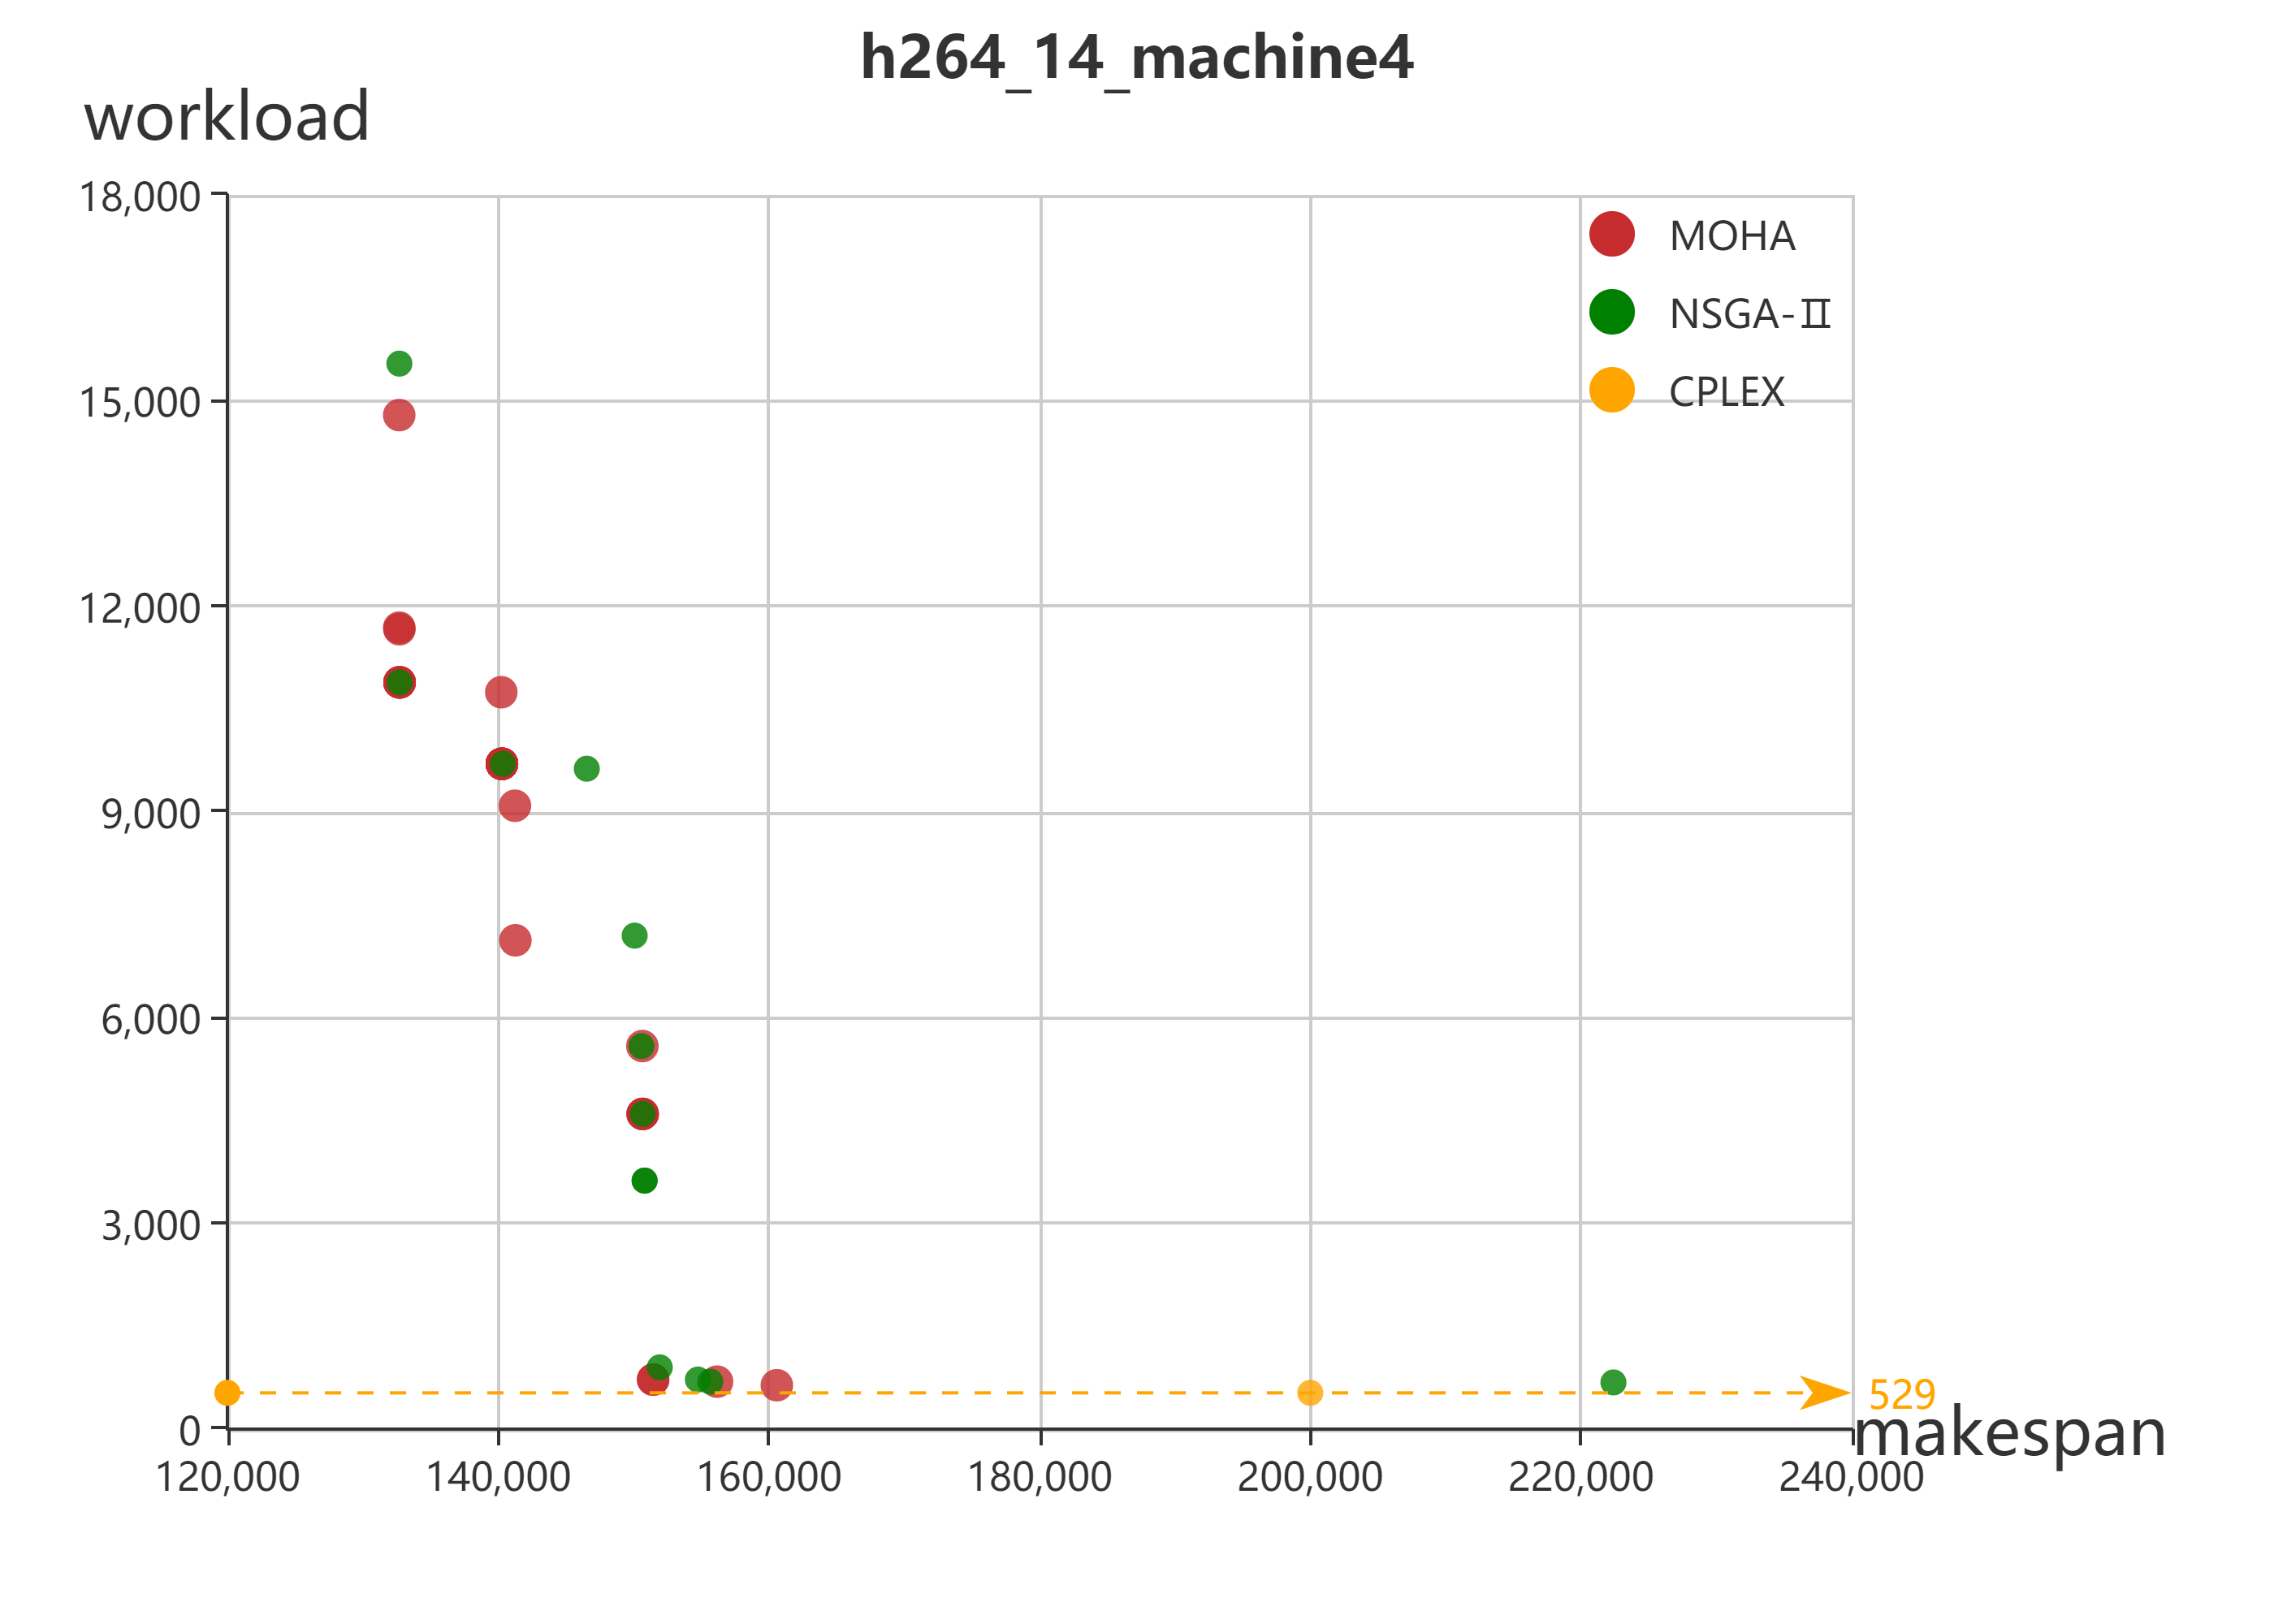
\includegraphics{./figures/h264_14_machine4}}}
%  
%%\end{minipage}}\
%}
%\caption{\label{fig:distribution}\rjnote Distribution of final sets obtained by MOHA and NSGAII}
% \end{figure} 

To evaluate the efficiency of our method, we have compared with the results from multi-objective evolutionary algorithm NSGAII~\cite{deb2002fast} and CPLEX over small scale examples. To compare with CPLEX, the two objectives are transformed into one by the introduced weights, whose ratios are sampled from (1:1) to (1:9999) and (9999:1) respectively. As the timeout of CPLEX is set to 2 hours, we could only obtain its results within the scale of 20 tasks and 2 processors.

%Two performance metrics are adopted to measure the effectiveness of the algorithm.
 
%The first one is an intuitive distribution of the non-dominated solutions which have been generated. 
The Pareto fronts\footnote{As the precedent relations are simple in these benchmarks, we could only obtain a few solutions in the Pareto fronts. } of the coarse-grained H264 decoder generated by MOHA, CPLEX and NSGAII, are illustrated in Fig. \ref{fig:distribution}. 
In the figure, the boundary of the two objectives are obtained by separated optimization for makespan and workload with CPLEX. 
And its Pareto fronts are calculated with various combination of weights.
%As Cplex can get only one solution after numerous of iterations, different weight combinations of the two objectives compose the Pareto front.
 %Also, the boundary of the two objectives are given by separately optimize makespan and workload using Cplex. 
We can observe that the results of MOHA are closer to the Pareto-front than that of NSGAII, and they can reach some boundaries computed by CPLEX. % on every benchmark. 

%What calls for special attention is that the dependency of tasks is so sequential in these instances that the pareto fronts only contain a few of solutions. However, it does not obstruct the observation of dominance.

Additional to the comparison from the figure, we also present the comparison from Set Coverage (C-metric), which reflects the degree of dominance is measured between different algorithms.
 Let \textit{X} and \textit{Y} be two approximations of the Pareto-front of a multi-objective problems. We define $C({A},{B})$ as the percentage of the solutions in \textit{B} that are dominated by at least one solution in \textit{A}, where
\begin{equation}
   C({A},{B})={\dfrac{u\in{B}|\exists v \in A: v \preceq u}{B}}.
\end{equation}
The higher $C({A},{B})$ is, the deeper extent $A$ dominates $B$.

The results of C-metric are listed in Table \ref{tab:cmetric}. $NA$ means the results are un-available within 2 hours.  As we can see, most solutions in MOHA dominate both NSGAII and CPLEX. 


%A second indicator called Set Coverage (C-metric) which reflects the degree of dominance is measured between MOHA and  NSGAII. Let \textit{X} and \textit{Y} be two approximations of the preto-front of an multi-objective problems,
%\begin{equation}
%   C({A},{B})={\dfrac{u\in{B}|\exists v \in A: v \preceq u}{B}}
%\end{equation}
%which is defined as the percentage of the solutions in \textit{B} that are dominated by at least one solution in \textit{A}. 
%/As Cplex can get only one solution after numerous of iterations, the metrics mentioned above are unapt. So, the third metric, \textit{W}(Cplex, MOHA), is whether the solution got by Cplex is dominated by the results of MOHA. In addition, the runtime \textit{Rtime} , solution numbers \emph{NumS} are also listed in TABLE \ref{tab:cplex}. The objective functions of Cplex are makespan and workload separately. That means for each instance, Cplex is run twice to optimize firstly the makespan and secondly the  workload. Results show that our proposed method gains no worse results than Cplex but spends less time in verse.
 
 \begin{table}[htp]\centering
\caption{Coverage Values between MOHA, CPLEX, NSGAII  \label{tab:cmetric}}%on six instances
\begin{lrbox}{\tablebox}
%\begin{scriptsize}
\begin{tabular}{|c|c|c|c|c|c|c|}
\hline

	\multirow{2}{*} {Benchmark} & \multirow{2}{*} {Tasks} & \multirow{2}{*} {Processors} & C(MOHA, & C(NSGAII,  & C(MOHA, & C(CPLEX,\\
	                  &           &               & NSGAII)  &  MOHA) & CPLEX) & MOHA) \\
\hline
	 \multirow{2}{*} {mp3decoder} &\multirow{2}{*}{16} & 2 & 0.8 & 0.2 & 1 & 0 \\
	 & & 4 & 0 & 0 & 1 & 0 \\ \hline
	\multirow{2}{*}{h264-14} & \multirow{2}{*}{14} & 2 & 0.4 & 0.17 & 0 & 0 \\
	& &   4 & 0.58 & 0.15 & 0 & 0\\ \hline
	\multirow{2}{*} {MWD} & \multirow{2}{*}{  12 } & 2 & 0 & 0 & 1 & 0\\
	& & 4 & 0 & 1 & 1 & 0\\\hline
	\multirow{2}{*}{TMNR} &\multirow{2}{*}{ 14 } & 2 & 0.67 & 0 & 0.5 & 0.5\\
	 && 4 & 0 & 0 & 0 &0.75\\\hline
	\multirow{2}{*}{FFT-loop} &\multirow{2}{*}{ 28} & 2 & 0.67 & 0.33 & 1 & 0\\

	& & 4 & 0 & 0.33 &NA &NA\\ \hline
	\multirow{2}{*}{FFT-butterfly} &\multirow{2}{*}{ 32} & 2  & 1 & 0 &NA &NA\\ 
        & 	& 4 & 1 &0 &NA &NA\\
%	mp3decoder & $ 16$ & 
%	h264-14 & $14$ & 4 & 0.58 & 0.15 & 0 & 0\\
%	MWD & $  12 $ & 4 & 0 & 1 & 1 & 0\\
%	TMNR & $ 14 $ & 4 & 0 & 0 & 0 &0.75\\
%	FFT-loop & $ 28 $ & 4 & 0 & 0.33 &NA &NA\\
%	FFT-butterfly & $ 32$ & 4 & 1 &0 &NA &NA\\
\hline
\end{tabular}	
%\end{scriptsize}
\end{lrbox}
\scalebox{0.65}{\usebox{\tablebox}}
\end{table}



% \begin{table}[htp]\centering
%\caption{Comparasion between Cplex and MOHA \label{tab:cplex}}
%\begin{lrbox}{\tablebox}
%\begin{tabular}{|c|c|c|c|c|}
%\hline
%	Dataset Name & Scale & W(Cplex, MOHA) & Rtime(s) & NumS %\\
%\hline
%	mp3decoder & $3 \ast 16$ & 0.75 & 0 & 1 \\
%	h264-14 & $2 \ast 14$ & 0.25 & 0.25 &1  \\
%	MWD & $3 \ast 12 $ & 1 & 0 & 1 \\
%	TMNR & $3 \ast 14 $ & 1 & 0 & 1 \\
%	FFT-loop & $2 \ast 28 $ & 1 & 0 &1 \\
%	FFT-butterfly & $2 \ast 32$ & 1 & 0 &1\\
%\hline
%\end{tabular}	
%\end{lrbox}
%\scalebox{0.9}{\usebox{\tablebox}}
%\end{table}
\subsection{ The scaliability of the MOHA algorithm}
\begin{figure}[htp]
\centering
	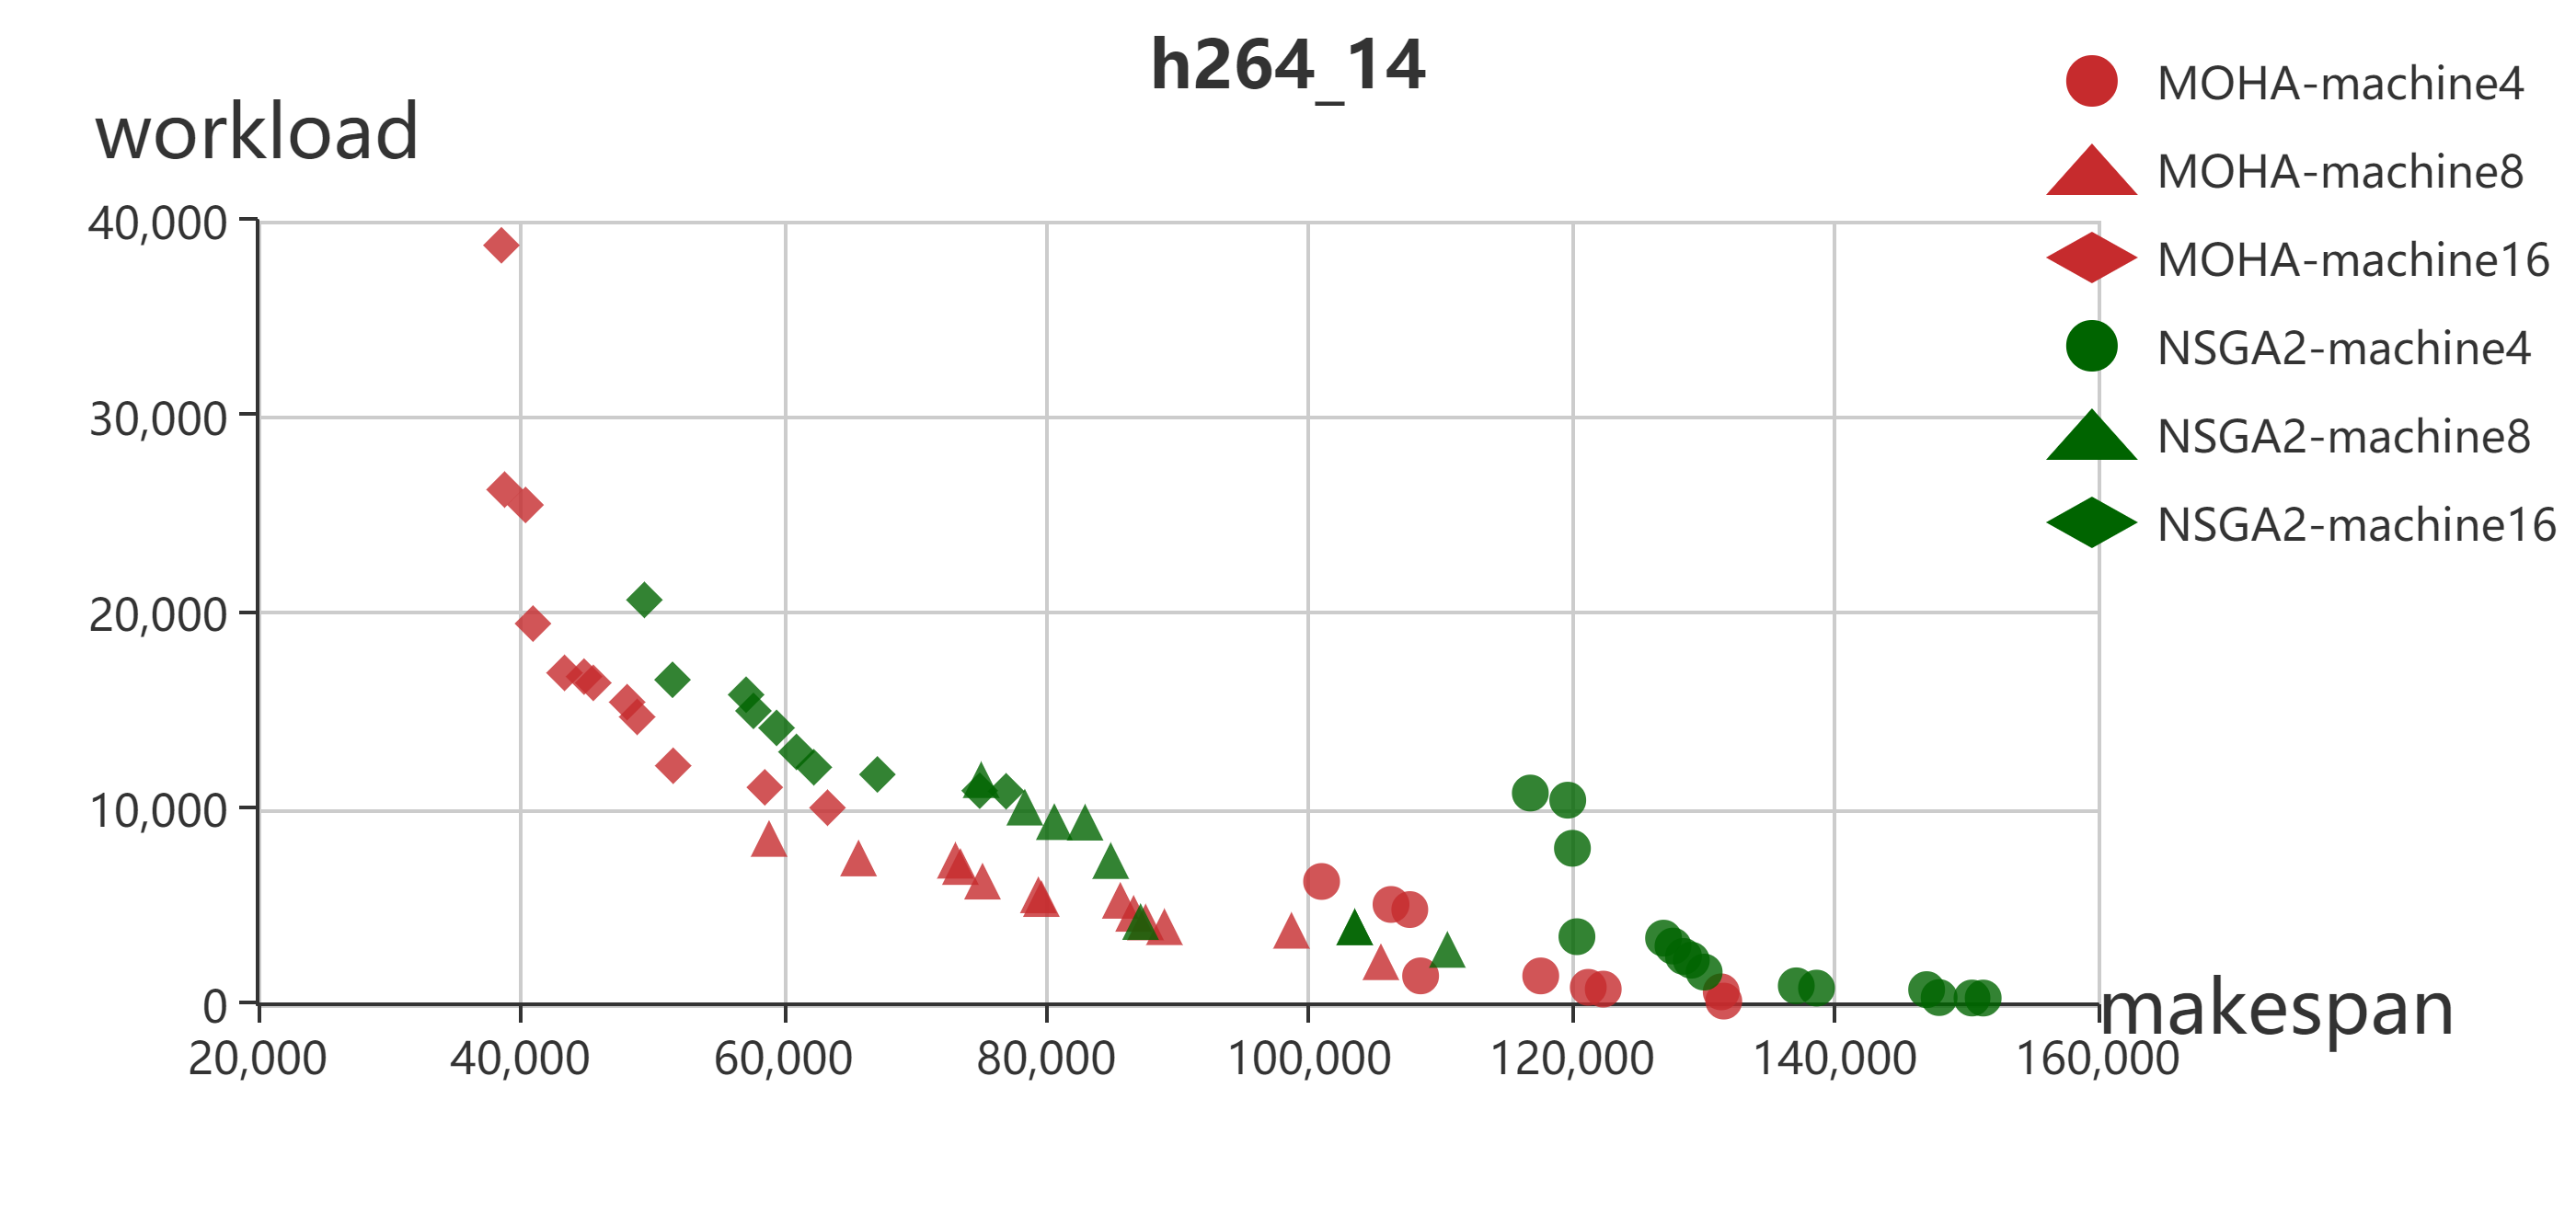
\includegraphics[width=0.9\columnwidth]{./figures/h264_14}
\caption{Distribution of final sets  for fine-grained H264}
 \label{fig:finegrained}
\vspace{-4mm}
 \end{figure} 
To show the scalability of our method, we have also evaluated the performance with the fine-grained H264 decoder example, with 264 tasks and 4, 8, 16 processors respectively. Its comparison with NSGAII is illustrated  in Fig. \ref{fig:finegrained}. The results show that MOHA can gain better results even on the large scale applications. 

%\subsection{Experimental Results}

